%!TEX root = thesis.tex

\chapter{Literature Review}
\label{chap:literature-review}

Visualisation is building momentum within the space of live coding. This chapter seeks to identify the reason for this momentum and identify the purpose and potential for visualisations within this field.

\section{Software}

Understanding changing software has been identified as one of the most important goals in software engineering practice~\cite{Tao2012}. It is the nature of software to change~\cite{Brooks1995} and there is a need for not only the programmer to understand the software but also for knowledge transfer to take place between those modifying the software and those impacted by the changes~\cite{Tao2012}.

Programming languages are the formal languages of software. These languages are typically represented by source code in a plain text format. However, plain text format is limited, requiring an interpretation step (parsing and compilation) to achieve a functioning program that can be understood by the computer~\cite{Badros2000}. The same occurs while programming. The programmer needs to comprehend the source code in order to make informed changes. In this case, the programmer conducts the interpretation step within the brain, rather than the computer, through a process of hypothesis creation, confirmation and refinement~\cite{Brooks1983}.

The steps involved in, and the issues with, interpreting and comprehending source code have been comprehensively examined within the literature (see ~\cite{Novais2013,McLean2010a,Brooks1995,Desmond,Rajlich2002}). Nevertheless, although many studies discuss the limitations of text-based source code, comparatively few have conducted empirical user studies examining the effectiveness of alternative representations of source code.

The concept of alternative source code representations is not new. Alternative representations of the source code include diagrams~\cite{Rumbaugh2004}, visual languages~\cite{Cox2007} and combinations of the two (e.g.~\cite{Lucanin2011}). Modern software development environments may also include tools that allow for alternative representations of code~\cite{Cox2007}. Diagrams, visual languages and modern software development environments vary greatly in relation to the source code with visualisations representing many levels of abstraction~\cite{Jerding1997}. Despite the differences in the level of abstraction and goal of the alternative representations, these approaches are all related through their common use of visualisation techniques.

\section{Visualisation}

Visualisation is widely understood as ``the use of computer-supported, interactive, visual representations of data to amplify cognition''~\cite{Card1999}. Further extensions of this definition discuss the need to perform cognitive work more efficiently~\cite{Ware2013a} and the need to transfer knowledge~\cite{Burkhard}. These definitions are summarised in the model shown in Figure~\ref{fig:model-of-visualisation}. This model shows the feedback loop attributed to a change in knowledge. Changes to knowledge impact perception but may also effect the user's exploration of the visualisation.

\begin{figure}
  \centering 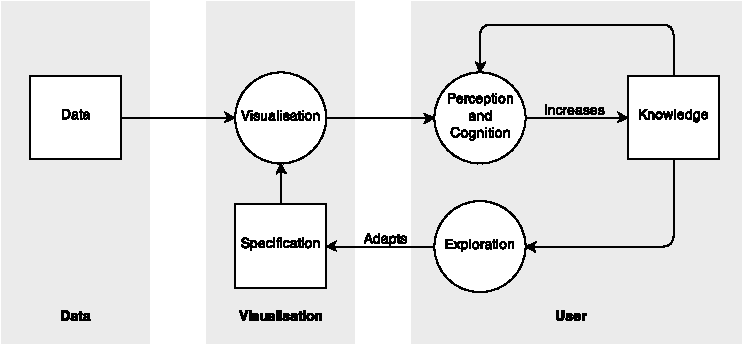
\includegraphics[width=\columnwidth]{../images/diagrams/wijk-model-of-visualisation.pdf}
  \caption[Generic model of visualisation]{Generic model of visualisation \protect\cite{VanWijk2005}.}
\label{fig:model-of-visualisation}
\end{figure}

Software visualisation is the process of representing the characteristics of computer programs visually~\cite{Stasko1992} in order to improve understanding~\cite{Diehl2007}. The advantage of providing a visual representation over the more traditional text-based representation is that the text-based approach does not take full advantage of human visual information processing capabilities~\cite{Myers1989}.

Initial efforts to classify software visualisations identified two axes: whether the visualisation illustrated the code, the data or the algorithm; and whether the visualisation was static or dynamic~\cite{Myers1989}. Taxonomies characterised software visualisations according to the aspect of the program, the abstractness of the visualisation, the animation and the automation of the visualisation~\cite{Stasko1992}.

Although it is the nature of software to change, static diagrams have traditionally been used to represent software systems visually. These diagrams typically show the structure (class diagrams) or function (state diagrams) of a software system at a specific moment in time~\cite{Rumbaugh2004}. The usefulness of these diagrams lies in their ability to represent fundamental structures within the program more concisely than the source code itself. However, it is not possible to represent a program's behaviour using these types of static diagrams~\cite{Baecker1998} and it is difficult to represent the evolution of the software using nothing but static diagrams.

Approaches to dealing with the visualisation of software evolution and realtime feedback have been integrated into modern software development environments. Modern software development systems and \acp{IDE} may feature syntax highlighting to assist in comprehension~\cite{Chen2005,Reis}, source code annotations, and the generation of visualisations based on the source code~\cite{Hendrix2004}, and allow the programmer to interact with the running program. These modern \acp{IDE} emphasise the relationship between the source code and the running program but are still fundamentally tools for source code manipulation.

Only the initial steps have been taken in order to implement and evaluate methods of communicating source code intent outside the field of programmer comprehension. Studies hint at the limitations of static diagrams, visual languages and modern software development environments and identify the need for alternative software representations and evaluation of their effectiveness for those with limited programming knowledge and experience. 

Visualisations have the capacity to present information more effectively than traditional programming languages. Nevertheless, software visualisations still require significant development to provide a benefit to the observers in the understanding of the complexity of software ~\cite{Baecker1995}. Effective software visualisations contribute to making software easier to understand, reflecting the software's history through the lifecycle, facilitating the transfer of knowledge from the programmer to the observer, making important structures visible and managing software complexity~\cite{Baecker1995}.

In a process-oriented activity such as live coding, different code visualisation techniques are necessary~\cite{McLean2010a,Magnusson2013}. However, these academic treatments of code visualisation in live coding adopt a survey-based approach, and the techniques discussed have not been subject to empirical evaluation.

\section{The Programmer and the Observer}

The relationship between the programmer and the observer has significant implications not just within the field of live coding but also within software engineering practice.

Commonly within live coding, the live coding artist is performing in front of an audience. This setup includes the live coder as the programmer and the audience as a passive observer. Similar structures occur within software engineering practice in pair programming and with the concept of the maintenance programmer~\cite{Robson1991}. In this case, rather than a passive role, the observer takes the active role of communicating mistakes or considering new ideas. Due to the similarities between these two fields, there is potential to apply software engineering techniques to the live coding process, and the potential to generalise the examination of live coding to software engineering practice.

In the literature, live coding audiences are yet to be surveyed as to whether the projected code within a live coding performance gives a greater sense of communication between the programmer and observer or a greater sense of alienation~\cite{Mclean2011}. Similarly, studies are yet to be conducted to determine if source code is the best way of communicating the programming process.

\section{Measuring Audiences' Experiences}

There is currently a search for software visualisations that increase enjoyment and understanding~\cite{McLean2010a}. Here enjoyment refers to the perceived benefit gained from observing the visualisations regardless of the level of understanding. Understanding refers to the ability of an observer or audience to comprehend the abstract thinking process of the programmer.

Enjoyment is the most common reaction to the positive effect of media~\cite{Vorderer2004}. Increased enjoyment is usually characterised by ``pleasurable affective response to a stimulus''~\cite{Brock2004} and is one of the fundamental goals of the modern media entertainment industry. Enjoyment, and the closely related concept of entertainment, are characterised or caused by a wide range of emotional responses including exhilaration, suspense, aesthetic appeal and a sense of achievement~\cite{Vorderer2004}. The literature identifies that further investigation into how design impacts enjoyment is needed~\cite{Reed1999}.

Understanding of a particular program is said to be achieved when the program can be explained ``in terms that are qualitatively different from the tokens used to construct the source code''~\cite{Biggerstaff1994}. Source code comprehension has a large body of research both within the understanding of text-based source code and within the space of software visualisation~\cite{Hosking2005}. In the space of live coding, this understanding is required to avoid a sense of distraction or exclusion~\cite{McLean2010a}. Measuring understanding could identify methods to reduce distraction and exclusion and provide a method to evaluate live coding.

Enjoyment and understanding align closely with the concepts of aestheticism and didacticism. Didacticism refers to the ultimate goal of teaching. This approach mirrors the concept of understanding from the previous section. A didactic approach intends to increase the level of understanding. Aestheticism refers to the ultimate goal of appealing to the senses. This approach mirrors the concept of enjoyment from the previous section. An aesthetic approach intends to increase visualisation usability and increase retention~\cite{Cawthon2007}. 

A wide variety of terms exist for describing phenomena related to aestheticism and didacticism. Expressiveness and effectiveness~\cite{Hundhausen1996,Hundhausen2002}, the aesthetic and the pragmatic~\cite{Angeli2006}, and the artistic and the pragmatic~\cite{Kosara2007} are similar concepts and comprehensively covered in regards to software visualisation, music visualisation, usability and preference.

Software visualisations within the space of live coding have the potential to manipulate these two variables~\cite{Iru,McLean2010a}. For example, by increasing visual interest it may be possible to increase aesthetic appeal, though increasing aesthetic appeal may reduce didacticism with increased visual complexity causing confusion.

The educational aspects of software visualisations have been examined in a number of studies~\cite{Baecker1998,Hundhausen2007} though few have applied these visualisations to areas outside the field of software engineering and fewer still have investigated software visualisations targeted at those with no programming experience.

There has been an initial examination of the aesthetics in graph drawing~\cite{Purchase1996,Purchase2001} and within the space of information visualisations~\cite{Cawthon2007,Bell}, though no studies have examined the effectiveness of process-driven software visualisations. This is particularly the case for the examination of live coded visualisations and the effect on audiences.

Some frameworks for both aesthetic evaluation of visualisations~\cite{Cawthon2007,Purchase1996} and didactic evaluation of visualisations~\cite{VanWijk2005} have been developed, though a thorough evaluation of the combination of the two concepts has not been considered.

\section{Future Directions}

Chapter~\ref{chap:introduction} identified the need for enhancing audience's experience within live coding. The literature discussed here demonstrates that those involved in live coding are looking for new and interesting ways of approaching this problem. The visualisation of software is not a new technique for enhancing the audience's experience but no empirical evaluations of the application of visualisation to live coding have been conducted.

Regarding the visualisation of live code, the most important questions identified include ``how can visualisations be applied to live coding?'' and ``what should be used as the metric to measure the success of the application of visualisations?''. Furthermore, the limitations of the current methods of software visualisation in general have been identified including how to best visualise the process of programming, how to visualise the evolution of software~\cite{Gall1999} and how to improve understanding and enjoyment of programming.

The model in Figure~\ref{fig:model-of-visualisation} and the investigation of the literature in this chapter identify some limitations in the current understanding and evaluation of visualisations. Firstly, within this model, a gain in knowledge is the only measurement of value and the only identified method for increased cognitive performance and increased exploration. Secondly, this model of visualisation inherently describes \textit{interactive} visualisations, where increased exploration allows for the adaptation of the specification. Many visualisations may not allow for an adaptation step to take place. 

The literature has identified that there may be more metrics appropriate for the evaluation of visualisations. Furthermore, live coding appears to be a space in which it may be possible to apply this model as a \textit{process} in the development of visualisations. Perhaps the exploration phases of this model could be adapted to meet the challenge presented within live coding to develop methods of source code visualisation that enhance the audience's experience, iteratively developing and adapting effective visualisation techniques.

Questions identified through the introduction (Chapter~\ref{chap:introduction}) and the literature review include, ``why show the source code at all during a live coding performance?'' and ``are there better methods of demonstrating the programming process?''. Systematic and empirical studies are yet to be conducted within live coding to answer these questions. Similarly, no studies have been conducted to evaluate effective metrics for analysis of the live coding process and the display of source code or visuals.

In an attempt to answer some of the questions raised, an exploratory field study was conducted (see Chapter~\ref{chap:exploratory-field-study}) in an effort to define the direction of the development and implementation of software visualisations within live coding.

